\FloatBarrier
\subsection{Executive Summary}
%\emph{Responsible:   WP3 coordinator, A. Freise   \\}

The optical design of the Einstein Telescope refers to the design of
the laser interferometer, the core instrument in which the
effect of a passing gravitational wave is
transformed into a read-out signal, measuring the changes 
in the distance between suspended mirrors using ultra-stable
laser beams. The amplitude of this signal
scales at first linearly with the light power stored in the  
interferometer arms. This led to the development of long-baseline
detectors utilising high-power lasers. The interferometers of 
first generation GW detectors were already extremely sensitive 
to arm length changes (and thus to gravitational waves). Their sensitivity
over a wide frequency range was limited not by technical inaccuracies 
but by intrinsic noise of their fundamental parts, such as the quantum
fluctuation of the laser light. The optical design efforts since then
have focused on developing and implementing advanced
optical technologies to reduce the impact of these noise sources 
on the read-out signal.

Gravitational waves exist in two distinct polarisations. To capture the
full signal a GW observatory should be able to detect both polarisations at
all times. This can be achieved by employing multiple co-located
detectors. The optimal footprint of the observatory will depend on the
geographical details of the yet unknown location. It is possible to
position three detectors in a triangle as shown in Figure~\ref{fig:ET_full_triangle}.
Such a triangular shape represents the minimal topological solution and
has been chosen as the baseline geometry for ET.
\begin{figure}[h]
	\centering
		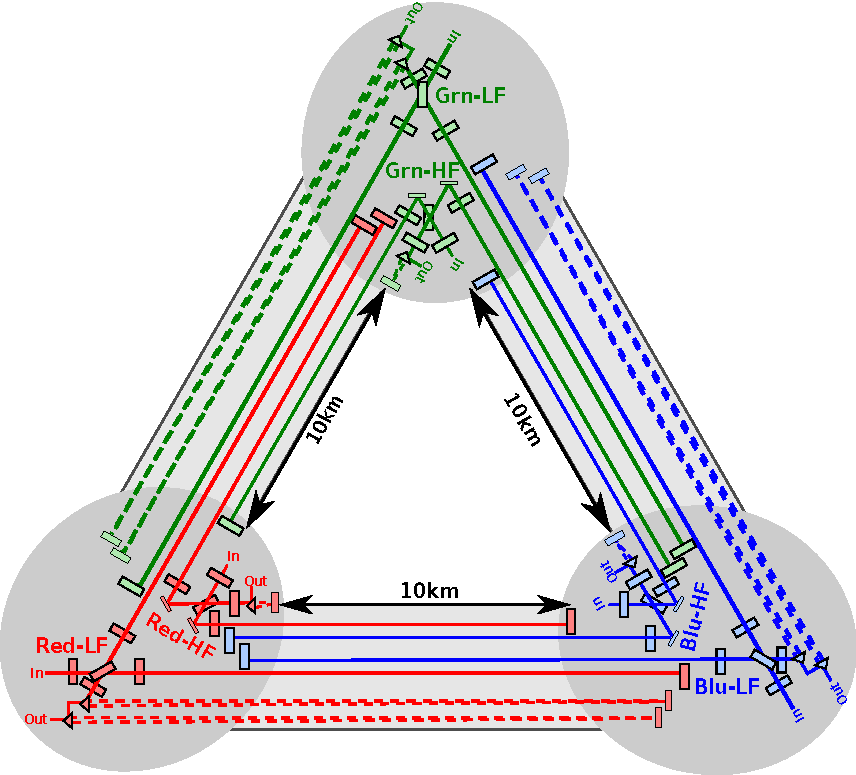
\includegraphics[width=0.6\textwidth]{Sec_Optics/ET_full_april2011.pdf}
	\caption{Schematic full view of the optical layout of the ET
    Observatory. 
 the full instrument consists of 3 pairs of km-scale
    interferometers positioned such that they form a triangular
    shape. Each interferometer pair represents one wide-band detector,
    in which one interferometer is optimised for gravitational waves
    at low frequencies (LF) and the other for high frequencies (HF).
Please note that this graphic is not too scale and does not show the exact position of the
optical components. Instead, it provides an overview of the general shape and
complexity of the optical layout of the main interferometers.
}
	\label{fig:ET_full_triangle}
\end{figure}

The core interferometers of the Einstein Telescope will be advanced
Michelson interferometers
with an arm length of 10\,km, a length which was a given input
parameters for the optical design. Some technologies for noise
reduction are not necessarily compatible with each other. Therefore
the optical design includes two parallel, 10\,km long interferometers per detector,
one interferometer being optimised for low-frequency (LF) gravitational
waves, the other covering the high frequency (HF) part of the spectrum; 
this approach has been called `xylophone' design.
The main characteristics of the two interferometer types are:
\begin{itemize}
\item the \textbf{HF} interferometer is a room temperature
  interferometer with very high laser power and fused silica test
  masses similar to Advanced
  detectors, but using an alternative laser beam shape,
the Laguerre-Gauss LG33 mode.
\item the \textbf{LF} interferometer is a cryogenic
  interferometer with medium laser power, using silicon test
  masses and a laser system with a 1550\,nm wavelength.
\end{itemize}

One of the main noise sources to suppress by means of optical
design is the quantum noise of the light.
A detailed study of newly proposed schemes for quantum
noise reduction, such as speed meters or optical bars has been
undertaken and two interesting candidates have been identified:
the ET baseline design will make use of dual-recycled Michelson
interferometers, very similar to those planned for Advanced LIGO, with
the additional injection of frequency-dependent squeezed light 
into the dark port. In parallel, we will continue to study speed-meter
like configurations, in particular those based on the Sagnac topology.

The choice of using Michelson interferometers (with recycling techniques) has the
great advantage that much of the research and development towards
the Advanced detectors can be applied directly. In particular, for the
conceptual designs of auxiliary systems such as input-output optics, 
the interferometer control or the thermal control of the
interferometer mirrors, we can adapt the current state of the art
with only small envisaged changes.

\vspace{5mm}
A summary of all the optical parameters of the Einstein Telescope
baseline design is given in the table below:
\begin{longtable}{p{5.5cm} *{2}{p{5cm}}}
	%%% HEADER, repeats on every page
	&	 \textbf{ET-HF}   	&	 \textbf{ET-LF} 	\\
\noalign{\smallskip}\hline\hline\noalign{\smallskip}
\endhead

%%% generic parameters for the whole itf
Approximate frequency range	&	10--$10^4$\,Hz 	&	1--250\,Hz	\\
Detection scheme	&	DC readout	& DC readout	\\
Input power (after IMC) 	&	500\,W 	&	3\,W 	\\
Laser wavelength 	&	1064\,nm 	&	1550\,nm 	\\
Beam shape 	&	LG$_{33}$	&	TEM$_{00}$	\\

%%% ARM CAVITIES
\noalign{\smallskip}\hline\noalign{\smallskip}					
\multicolumn{3}{c}{\textit{ARM CAVITIES}}	\\				
\noalign{\smallskip}\hline\noalign{\smallskip}					

Arm length 	&	10\,km	&	10\,km 	\\
Opening angle	&	$60\,^\circ$	&	$60\,^\circ$	\\
Arm power 	&	3\,MW 	&	18\,kW	\\
Temperature 	&	290\,K 	&	10\,K  	\\
Mirror material 	&	fused silica 	&	silicon  	\\
Mirror diameter	&	62\,cm	&	>45\,cm	\\
Mirror thickness 	&	30\,cm	&	about 50\,cm	\\
Mirror mass	&	200\,kg 	&	211\,kg 	\\
Beam radius (at mirror)	&	7.2\,cm 	&	9.0\,cm	\\
Beam waist (symmetric cavity)	&	2.51\,cm	&	2.9\,cm	\\
RoC (symmetric cavity)	&	5690\,m	&	5580\,m	\\
%Rayleigh range (symmetric cavity)	&	1860\,m	&	1700\,m	\\
Scatter loss per surface 	&	37.5\,ppm 	&	37.5\,ppm 	\\
Finesse	&	880		&	880		\\
Reflective coating ITM	&	tantala/silica	&	tantala/silica	\\
	& 	8 $\lambda/4$ doublets	&	9 $\lambda/4$ doublets	\\
Reflective coating ETM	&	tantala/silica	&	tantala/silica	\\
	&	17 $\lambda/4$ doublets	&	18 $\lambda/4$ doublets	\\
Transmission ITM	&	7000\,ppm	&	7000\,ppm	\\
Transmission ETM	&	6\,ppm	&	6\,ppm	\\

%%% CENTRAL INTERFEROMETER
\noalign{\smallskip}\hline\noalign{\smallskip}					
\multicolumn{3}{c}{\textit{CENTRAL INTERFEROMETER}}	\\				
\noalign{\smallskip}\hline\noalign{\smallskip}					

SR-phase 	&	tuned (0.0) 	&	detuned (0.6)	\\
Focussing element	&	in or near the ITM 	&	in or near the ITM	\\
                	& 	focal length $= 303$\,m	&	focal length $= 303$\,m	\\
Distance ITM--BS	&	300\,m	&	300\,m	\\
Distance BS--MPR	&	10\,m	&	10\,m	\\
Recycling cavity length	&	310\,m	&	310\,m	\\
Beam size on BS	&	4.7\,mm	&	6\,mm	\\
Beam size on MPR	&	2.7\,mm	&	3.4\,mm	\\
Recycling gain	&	21.6	&	21.6	\\
Recycling cavity free spectral range	&	484\,kHz	&	484\,kHz	\\
%Rayleigh range in central IFO	&	40\,m	&	47.0\,m	\\
Round-trip Guoy phase	&	$10.5\,^\circ$	&	$9.6\,^\circ$	\\
mode separation frequency	&	28\,kHz	&	26\,kHz	\\
Recycling cavity temperature	&	room temperature	&	room temperature	\\
Beam splitter material	&	fused silica	&	fused silica	\\
%Beam splitter diameter	&	?	&	around 50\,cm	\\
%Beam splitter thickness	&	?	&	about 30\,cm	\\
%Beam splitter coating	&	?	&	tantala/silica	\\
%	&	&	3 $\lambda/4$ doublets (upper limit)	\\
Transmission PRM	&	4.6\,\%	&	4.6\,\%	\\
Transmission SRM	&	10\,\% 	&	20\,\% 	\\

%%% FILTER CAVITIES
\noalign{\smallskip}\hline\noalign{\smallskip}					
\multicolumn{3}{c}{\textit{FILTER CAVITIES}}	\\				
\noalign{\smallskip}\hline\noalign{\smallskip}					
Quantum noise suppression 	&	frequency-dependent squeezing	&	frequency-dependent squeezing	\\
Filter cavities 	&	$1 \times 300\,$m  	&	$2 \times 10\,$km	\\
%Squeezing level  	&	refer to~\ref{fig:sqzHF} 	&	refer to Fig.~\ref{fig:sqz} 	\\
Half-bandwidth	&	5.7\,Hz	&	5.7\,Hz and 1.5\,Hz\\
%Resonance frequency	&	?	&	$2\pi\cdot 6.6\,Hz$ / $-2\pi\cdot 25.4\,Hz$	\\
Detuning	&	25.4\,Hz	&	25.4\,Hz and 6.6\,Hz\\
Round-trip loss	&	75\,ppm	&	75\,ppm	\\
%Coupling mirror reflectance	&	?	&	98.8864\% / 99.5323\%	\\
\noalign{\smallskip}\hline\noalign{\smallskip}					

%%% SUSPENSIONS
%\multicolumn{3}{c}{\textit{SUSPENSIONS}}	\\				
%\noalign{\smallskip}\hline\noalign{\smallskip}				
%Seismic isolation 	&	SA, 8\,m tall 	&	mod SA, 17\,m tall 	\\
%Seismic (for $f>1$\,Hz) 	&	$5\cdot 10^{-10}\,{\rm m}/f^2$ 	&	$5\cdot 10^{-10}\,{\rm m}/f^2$  	\\
%Gravity gradient subtraction 	&	none 	&	none 	\\
%\noalign{\smallskip}\hline\noalign{\smallskip}					
%\multicolumn{3}{c}{\textit{INJECTION OPTICS}}	\\				
%\noalign{\smallskip}\hline\noalign{\smallskip}					
%Intensity noise	&	TBD	&	TBD	\\
%Beam jitter noise	&	TBD	&	TBD	\\
%Overall throughput	&	$>50\%$	&	$>50\%$	\\
%IMC cavities	&	$2\times 20$\,m	&	$2\times 20$\,m	\\
%	&	even number of mirrors	&	triangular cavities	\\
%IMC cavities throughput	&	$>80\%$	&	$>80\%$	\\
%IMC mirrors substrate	&	fused silica 	&	?	\\
%IMC coating absorption	&	$<1$\,ppm	&	?	\\
%\noalign{\smallskip}\hline\noalign{\smallskip}					

%%% DETECTION OPTICS
% \multicolumn{3}{c}{\textit{DETECTION OPTICS}}	\\				
% \noalign{\smallskip}\hline\noalign{\smallskip}					
% Detection scheme	&	?	&	?	\\
% \noalign{\smallskip}\hline\noalign{\smallskip}					

\end{longtable}



%%% TODO: add more here, at least covering filter cavities and LG
%%% modes. Could also quickly run through the list of optical 
%%% parameters?





\FloatBarrier
\subsection{Description}
%\emph{Responsible:  WP3 coordinator, A. Freise  \\}

Modern gravitational wave detectors are based on km-scale laser interferometers.
Also the Einstein Telescope is using a sophisticated laser
interferometer
to convert the signal of a passing gravitational wave into a readout
signal that can be processed electronically. The basic
interferometer design is still similar to that of the original
interferometer by Michelson (used more than 100 years ago in the famous Michelson and Morley
experiment to disprove the existence of a so-called aether). However,
to achieve better sensitivities 
the interferometry has been refined and extended continuously, especially during
the last two decades, driven by the gravitational wave community. As a result, modern
interferometers are now able to reach unprecedented sensitives beyond the Standard
Quantum Limit of interferometry. At the same time the optical design
has become a more challenging task. Modern interferometers couple all
involved optical systems into one closely coupled, complex machine. 

The focus of the optical design was to identify and develop an optical layout for the
core interferometer of a third generation detector which includes
advanced optical technologies required to reach the target sensitivity
of the ET detector. The term `optical layout'  includes a number of
layers of complexity in optical design: first of all, the core
interferometer is the part of the detector which converts the
gravitational wave signal into a measurable optical signal. Second,
the core interferometer by design couples all auxiliary subsystems
together. Thus part of the effort in this design study was dedicated to how the
signal and all possible noises couple into the detector output.  And
third the optical layout largely defines the type of instrument,
i.e.\ it defines the shape of the detector, the type of interferometry
used, as well as which advanced optical technologies are included.

In order to achieve the envisaged sensitivity of the Einstein
Telescope, once again the interferometry must be pushed beyond
the state-of the art. For the first time a number of advanced
technologies such as cryogenic mirrors, squeezed light and 
alternative beam shapes are to be combined in one system.
This section describes in detail the design process towards the
optical layout of ET which forms the baseline for the design of the
infrastructure, as well as the mirror suspension systems.
%% --- adf
All the currently active GW detectors are L-shaped, with orthogonal
arms; although this geometry maximises the sensitivity of the single
detector with respect to the arm length, other geometries are
possible. In particular, triangular-shaped detectors have been
proposed in the past; the LISA geometry is also triangular.
 Two L-shaped
detectors, forming a 45 degrees angle, could fully resolve the two
polarisation amplitudes of the incoming wave. Obviously in an
underground site, the realization of this geometry is
difficult, due to the high cost of the infrastructure. If the angle
between the two arms of each
detector is reduced to 60 degrees, three detectors can be accommodated
in a triangular-shaped underground site, minimizing the required
number
of caverns. An
analysis of a triangular-shaped
third generation GW observatory is described in
sections~\ref{sec:georeview}
%and \ref{sec:toporeview} 
with the conclusion that if a site that can
accommodate a triangular observatory is found, 
the triple co-located interferometers will be the best choice and the
triangular shape has been adopted as the baseline for the current
ET design.

Each detector within a triangular observatory can in principle be composed of
one or several interferometers of different topology. It can be shown
that one interferometer per detector is not ideal.
Spanning the wide detection band envisaged for ET is technically
extremely challenging: Different noise types dominate the various
frequency bands and often these noises show opposite response for
changing the involved design parameters. Sometimes the reduction
techniques for different noise types are incompatible. 
A well-known example for a parameter that affects different frequency
regions differently is the correlation of the two quantum noise
components: photon shot noise and photon radiation pressure
noise. In order to improve the shotnoise-limited sensitivity at high
frequencies one needs to increase circulating optical power,
which at the same time increases the radiation pressure noise and therefore worsens
the low frequency sensitivity. Alternatively, lowering the circulating
power reduces the radiation pressure effects and improves the low frequency sensitivity,
while the shotnoise contribution will rise and reduce the high frequency
sensitivity. 
This dilemma can be resolved by following the path of electromagnetic
astronomy, where telescopes are being built for a specific, rather
narrow-banded detection window (visible, infrared etc) and later on
the data from different frequency bands are combined to cover the
desired bandwidth.  Building two interferometers, each optimised
for reducing the noise sources at one specific frequency band, can
form a xylophone observatory providing substantially improved
broadband sensitivity. 
We have developed a
2-band xylophone detector configuration to resolve the high-power
low-temperature problem of a single band ET observatory as described
in section~\ref{sec:optlayout}.  Based on this design envelope of
three xylophone detectors in a triangular setup, a more detailed
design of the optical layout can be performed. 
This formed the basis for the investigation into the required cavern
size and associated infrastructure impact,
see section~\ref{sec:SiteInfra}.

%%% Topology Choice, Quantum noise reduction, Squeezed light
Currently the Michelson interferometer topology is used in
laser-interferometric gravitational wave detectors. However,
alternative topologies, such as the Sagnac interferometer or so-called
`optical bars',  have been suggested and would also fit into a triangular, xylophone based detector. The main
attraction of alternative interferometer topologies is that
they allow the implementation of different quantum noise reduction
schemes. While classical interferometers are limited by the Standard
Quantum Limit, a noise floor composed of photon shotnoise and
radiation pressure effects, clever interferometer designs and the use
of squeezed light allow us to push beyond that limit. A detailed study 
of a wide range of possible quantum noise reduction schemes has
been undertaken and is reported in sections~\ref{sec:qnr} and
\ref{app:QNR}.
As the outcome of this study, taking into account technical considerations, a 
Michelson-based topology with Signal Recycling and squeezed light
injection has been selected for the Einstein Telescope baseline.
The study also showed that Sagnac-based speedmeter topologies are an appealing 
alternative and should be studied further.
The chosen design implements so-called filter cavities to generate the
frequency-dependent squeezed light. During the course of the design
study a lot of original research has been undertaken to derive
requirements for such cavities and their implementation, details
are reported in appendix~\ref{app:filtercavities}.

%%% Details
With the baseline of the optical layout selected, the design progressed
into essential subsystems. The core element of these laser
interferometers are the large principal mirrors of the arm
cavities. The
thermal noise of these mirrors represents one of the main limits to
the achievable sensitivity. Towards the realisation of
second-generation interferometric detectors, a major research effort
is underway to study and improve all aspects of these mirrors,
especially the quality of the dielectric coatings. This work has been
extended here to determine the requirements for the Einstein
Telescope. A further challenge is to identify the best material and
design choices for the cryogenic mirrors to be used in the
low-frequency interferometer. Two solution based on Sapphire and
silicon as mirror bulk material have been
identified and carefully studied in section~\ref{sec:optcomps} alongside
fused-silica mirrors for the high temperature interferometer. This
work is complemented by tables stating the optical, mechanical and thermal 
properties in appendix~\ref{sec:app}.

The following sections~\ref{sec:injection}, \ref{sec:detection}, \ref{sec:control}
and \ref{sec:tcs} provide details about auxiliary optics system, such as the
injection
optics, providing the laser beam to the main interferometer, the
detection system, responsible for converting optical into electrical
signals and the control systems required to maintain a stable
operating position of the entire interferometer. The design of these
systems is a direct application and extension of the work done 
and experience gained with the first and second generation of 
detectors and we expect future changes to these systems based
on the experience gained when the advanced detectors
start operating. 

Building on the detailed baseline design of the optical layout as well as
the main subsystems, section~\ref{sec:opti_costs}  provides a cost
evaluation of the optical
system for the Einstein Telescope. We also provide 
a guide to future R\&D activities by outlining in section~\ref{sec:RD} 
which of the technologies require
major R\&D efforts before they could be incorporated in a technical  
design of the Einstein Telescope.

%%% Alternative technologies

During the course of the design study we have also investigated a
number of new and hypothetical effects or technologies. One 
hypothesis that gained popularity for a while proposes a new kind of
noise originating 
from the holographic principle of unification physics, which can arise in the 
high-precision interferometry \cite{2009_holonoise}. We investigated
this so-called holographic 
noise (cf. Appendix~\ref{app:holo}) and came to the conclusion that it
is so far insufficiently developed and verified from both theoretical
and experimental sides, and we do not expect it to have any impact of
the design of ET. 
Further, a technique proposed to eliminate all types of
noise associated with the motion of test masses is the so-called
\emph{displacement-noise free interferometry}. Also this has been
investigated in Appendix~\ref{app:DFI}, but dismissed as it currently provides no route towards
a realistic experimental implementation. 